%************************************************
\chapter{Case Study}\label{ch:evaluation}
%************************************************
Part of the evaluation of the developed tool is to verify the functionality with an existing company. In order to do so, a company closely related to the University of Groningen has been found. This company is named `Sustainable Buildings' and sells products to monitor the users electricity and gas consumption in real-time. This leads to an increase in building-users awareness by providing real-time feedback through public dashboards \cite{sb}.\\

\noindent
In order to provide this monitoring, they have allocated a physical server consisting of 40 cores and 128 GB of RAM. Additionally, they have 900 GB of storage data. This host machine is divided into 6 virtual machines. A brief overview of their architecture is described in \autoref{sec:sb-architecture}. The decision has been made to deploy the developed tool at their system, because it is a relatively large system with many load. Additionally, the tool might be useful for them, as they are now missing insights into their performance. The process of deploying this system has been described in \autoref{sec:sb-process}. At the end, an evaluation has been performed. This evaluation consists of an interview and is described in \autoref{sec:sb-evaluation}.

\section{Architecture} \label{sec:sb-architecture}
The six virtual machines work together as one system. Each virtual machine is responsible for running a number of services. These services can be found in \autoref{fig:sb-architecture}. In order to simplify the deployment, the decided to assign a name to every VM. The names are also presented in the architecture diagram. A small overview of the number of CPU, RAM and memory per VM can be found in \autoref{tab:vms}.\\

As described in \autoref{sec:collect_utilization}, the architecture is a fully connected peer-to-peer system, as well as a hierarchical structure for the data replication. For the latter, the structure can be found in \autoref{fig:sb-tree}.


\begin{figure}
    \centering
    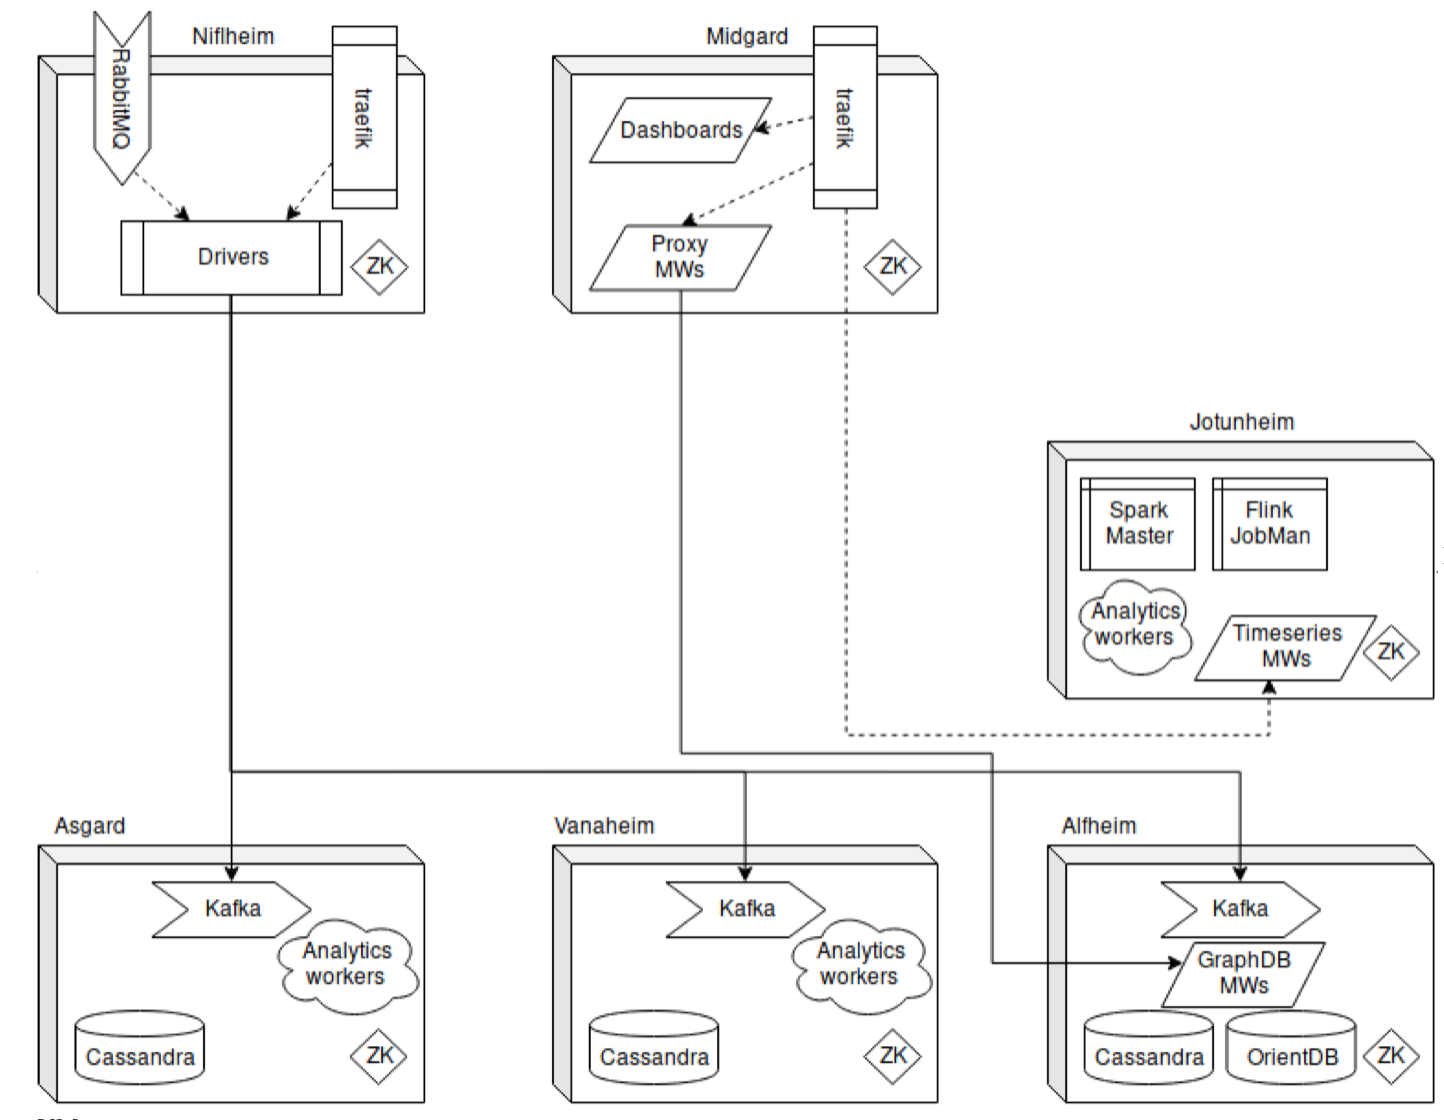
\includegraphics[width=\textwidth]{gfx/sb-architecture.png}
    \caption{Sustainable Buildings architecture}
    \label{fig:sb-architecture}
\end{figure}

\begin{table}
    \centering
    \begin{tabular}{l|rrr}
        Virtual Machine & Cores & RAM & Memory \\ \hline
        Midgard & 4 & 8 GB & 20 GB \\
        Niflheim & 4 & 8 GB & 20 GB \\
        Jotunheim & 8 & 16 GB & 100 GB \\
        Asgard & 8 & 16 GB & 100 GB \\
        Vanaheim & 8 & 16 GB & 100 GB \\
        Alfheim & 8 & 16 GB & 100 GB \\
    \end{tabular}
    \caption{Overview of their architecture}
    \label{tab:vms}
\end{table}

\begin{figure}
    \centering
    \begin{forest}
        for tree={
            grow=south,
            rectangle, draw, minimum size=3ex, inner sep=1pt,
            s sep=7mm
        }
        [Alfheim 
            [Vanaheim 
                [Asgard]
            ]
            [Midgard
                [Jotunheim]
                [Niffelheim]
            ]
        ]
    \end{forest}
    \caption{Hierarchical overview of the Case study}
    \label{fig:sb-tree}
\end{figure}


\section{Deployment process} \label{sec:sb-process}

\section{Evaluation} \label{sec:sb-evaluation}
